\section{The visualization layer}
In the visualization layer the system transforms the AST into a semantic Flow Graph that aligns with the user's mental model.
If the system would just naively display the nodes of the AST the Flow Graph would be strongly diffuse. Therefore the goal when transforming the AST is to reduce the overall number of nodes and edges while still preserving the semantics. %TODO: refer the diffuseness.

\subsection{Literals}
Literals for example numbers or strings, if presented as nodes they quickly cluster the Flow Graph without adding meaningful value for the user. The system solves this by not creating nodes for literals and instead placing them directly into their parent node. There they are still visible but do not occupy any additional space in the graph.
\subsection{Binary operations}
%TODO: Comparison images ???
\subsection{Cell References}
%TODO: add cell reference / range or is it the same ??
In order to understand the dependencies of the formula the system explicitly creates nodes for cell references. A cell reference node has tree important components. The most important component is the address component. The address is colored accordingly to the pre-defined color of its Sheet. When importing a new workbook the system generates distinct colors for each worksheet. The decision to color it by the respective worksheet was important because in a formula writing A2 automatically resolves the residing sheet of the address to where the formula resides. But when formulas refer across worksheets two distinct address can look the same even though they refer two different cells or ranges. The colors were used to add a secondary notation \cite{green_usability_1996} to resolve this problem see Figure \ref{fig:identical-address-formula} instead of text.

%TODO (IMPORTANT): update graphic if we change notations and make it prettier
\begin{figure}[htbp]
    \centering
    \begin{minipage}{0.45\textwidth}
        \centering
        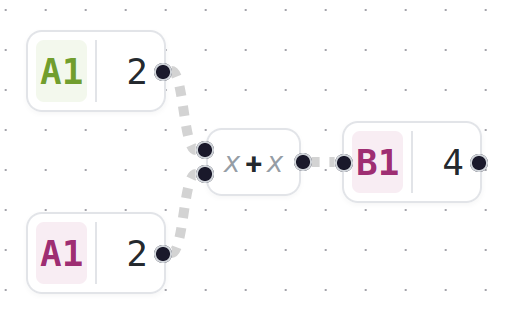
\includegraphics[width=\textwidth]{chapters/system-design/images/two-identical-looking-address-with-secondary-notation.png}
        \caption{First image}
        \label{fig:identical-address-formula}
    \end{minipage}
    \hfill
    \begin{minipage}{0.45\textwidth}
        \centering
        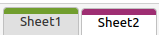
\includegraphics[width=\textwidth, scale=0.1]{chapters/system-design/images/sheet-tabs-colors.png}
        \caption{Second image}
        \label{fig:sheet-tabs-colors}
    \end{minipage}
\end{figure}

The second component of a reference node is its name. The system naively resolves names by getting the first string valued cell from the left and from the top. This naming system assumes that worksheets are organized by columns and each column has a different meaning and each row is a finer label of the column \cite{ivanova_introduction_2013}. The naming system can be improved in the future. 
The last component is the result component which displays the data the cell at the referenced address holds. This allows the user to quickly see without navigating inside the workbook to the cell the value is. 

\subsection{Functions}
\subsection{Conditional Nodes}
